\documentclass{beamer}
%Для защит онлайн лучше использовать разрешение 16x9
%\documentclass[aspectratio=169]{beamer}

% !TeX spellcheck = ru_RU
% !TEX root = vkr.tex
% Опциональные добавления используемых пакетов. Вполне может быть, что они вам не понадобятся, но в шаблоне приведены примеры их использования.
\usepackage{tikz} % Мощный пакет для создание рисунков, однако может очень сильно замедлять компиляцию
\usetikzlibrary{decorations.pathreplacing,calc,shapes,positioning,tikzmark}

% Библиотека для TikZ, которая генерирует отдельные файлы для каждого рисунка
% Позволяет ускорить компиляцию, однако имеет свои ограничения
% Например, ломает пример выделения кода в листинге из шаблона
% \usetikzlibrary{external}
% \tikzexternalize[prefix=figures/]

\newcounter{tmkcount}

\tikzset{
  use tikzmark/.style={
    remember picture,
    overlay,
    execute at end picture={
      \stepcounter{tmkcount}
    },
  },
  tikzmark suffix={-\thetmkcount}
}

\usepackage{booktabs} % Пакет для верстки "более книжных" таблиц, вполне годится для оформления результатов
% В шаблоне есть команда \multirowcell, которой нужен этот пакет.
\usepackage{multirow}
\usepackage{siunitx} % для таблиц с единицами измерений

\newcommand{\cd}[1]{\texttt{#1}}
\newcommand{\inbr}[1]{\left<#1\right>}

% Для названий стоит использовать \textsc{}
\newcommand{\OCaml}{\textsc{OCaml}}
\newcommand{\miniKanren}{\textsc{miniKanren}}
\newcommand{\BibTeX}{\textsc{BibTeX}}
\newcommand{\vsharp}{\textsc{V$\sharp$}}
\newcommand{\fsharp}{\textsc{F$\sharp$}}
\newcommand{\csharp}{\textsc{C$\sharp$}}
\newcommand{\GitHub}{\textsc{GitHub}}
\newcommand{\SMT}{\textsc{SMT}}

\newcolumntype{L}[1]{>{\raggedright\let\newline\\\arraybackslash\hspace{0pt}}m{#1}}
%\newcolumntype{C}[1]{>{\centering\let\newline\\\arraybackslash\hspace{0pt}}m{#1}}
\newcolumntype{R}[1]{>{\raggedleft\let\newline\\\arraybackslash\hspace{0pt}}m{#1}}

\usepackage{xcolor}

%  Команды и пакеты, не используемые в шаблоне, которые тем не менее могут быть полезными.

% \newcolumntype{Y}{>{\centering\arraybackslash}X}

% \usepackage{mathrsfs}

\lstdefinestyle{fsharp}{
  basicstyle=\small\ttfamily,
  keywordstyle=\color{blue},
  commentstyle=\color{lightblue},
  stringstyle=\color{red},
  numbers=left,
  numberstyle=\tiny\color{gray},
  stepnumber=1,
  numbersep=10pt,
  backgroundcolor=\color{white},
  showspaces=false,
  showstringspaces=false,
  showtabs=false,
  tabsize=2,
  breaklines=true,
  breakatwhitespace=false,
  morekeywords={async, let, rec, if, then, else, do, yield, return, use, match, with, function}
  literate={->}{{$\to$}}3 {==}{{$\equiv$}}1 {=/=}{{$\not\equiv$}}1 {|>}{{$\triangleright$}}3 {\\/}{{$\vee$}}2 {/\\}{{$\wedge$}}2 {>=}{{$\ge$}}1 {<=}{{$\le$}}
}


% То, что в квадратных скобках, отображается внизу по центру каждого слайда. 
\title[Процедурная генерация интерьера]{Реализация процедурной генерации интерьера комнат в 3D-игре на Unity}

% То, что в квадратных скобках, отображается в левом нижнем углу. 
\institute[СПбГУ]{}

% То, что в квадратных скобках, отображается в левом нижнем углу.
\author[Савельева Полина]{Савельева Полина Андреевна, группа 22.Б07-мм}
 
\begin{document}
{
\setbeamertemplate{footline}{}
% Лого университета или организации, отображается в шапке титульного листа
\begin{frame}
  
\includegraphics[width=1.4cm]{pictures/SPbGU_Logo.png}
\vspace{-35pt}
\hspace{-10pt}
\begin{center}
   \begin{tabular}{c}
        \scriptsize{Санкт-Петербургский государственный университет} \\
        \scriptsize{Кафедра системного программирования}
    \end{tabular}
\titlepage
\end{center}

\btVFill

{\scriptsize
  % У научного руководителя должна быть указана научная степень
   \textbf{Научный руководитель:} к.т.н. Ю.~В.~Литвинов, старший преподаватель кафедры системного программирования \\
  % Консультанта может и не быть. Должна быть указана должность или ученая степень
   \textbf{Консультант:}  Р.~А.~Береснёв, cтудент 3-го курса СПбГУ \\
 }
\begin{center}
  \vspace{5pt}
  \scriptsize{Санкт-Петербург\\
                 2023}
  \end{center}

\end{frame}
}

\begin{frame}[fragile]  
  \frametitle{Введение}
  \begin{itemize}
    \item Ручное заполнение комнат в игре Time Reactor является трудоемким процессом
    \item Процедурная генерация, PCG
    \begin{itemize}
        \item Создание разнообразного наполнения в больших масштабах
        \item Нет необходимости хранить данные
        \item Экономия времени
        \item Повторное использование генераторов
    \end{itemize}
    \item Процедурно генерируемое помещение
    \begin{itemize}
        \item Паттерны
        \item Временные ограничения
        \item Неизменность при повторном посещении
    \end{itemize}
  \end{itemize}
\end{frame}

% Обязательный слайд: четкая формулировка цели данной работы и постановка задачи
% Описание выносимых на защиту результатов, процесса или особенностей их достижения и т.д.
\begin{frame}
  \frametitle{Постановка задачи}
  \textbf{Цель}: реализация процедурной генерации интерьера комнат в игре Time Reactor на Unity %озвученной выше  

  \textbf{Задачи}:
  \begin{itemize}
    \item Изучение существующих решений
    \item Реализация библиотеки на .NET для процедурной генерации интерьера игровых комнат и ее публикация на NuGet
    \item Реализация процедурной генерации интерьера комнат в игре Time
Reactor на Unity с использованием разработанной библиотеки
    \item Проведение апробации среди заинтересованных игроков
  \end{itemize}
\end{frame}
            
\begin{frame}  
  \frametitle{Существующие решения}
  \vspace*{\fill}
  \begin{center}
        \begin{figure}
            \centering
            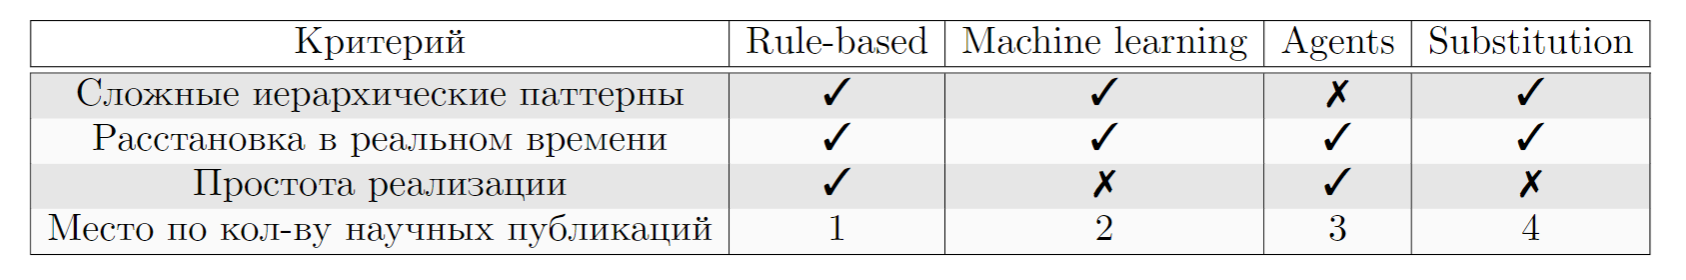
\includegraphics[width=1.0\textwidth]{pictures/comparison_table.png}
            \caption{Сравнение существующих решений\footnote{Данные о количественном отношении взяты из обзорной статьи \enquote{Recent Advances in Procedural Generation of Buildings: From Diversity to Integration}}}
        \end{figure}
  \end{center}
  \vspace*{\fill}
\end{frame}
            
%Идеально, если есть по одному слайду на каждую поставленную задачу            
\begin{frame}
  \frametitle{Основанный на правилах подход}
    \begin{figure}
      \centering
      \begin{minipage}{0.45\textwidth}
        \centering
        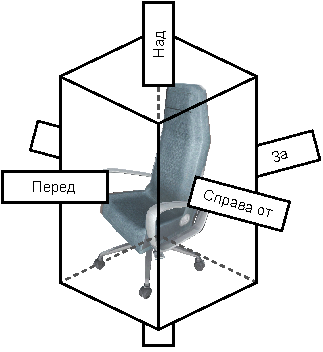
\includegraphics[width=0.5\textwidth]{pictures/collider.pdf}
        \caption{Ограничительная рамка у объектов}
      \end{minipage}
      \hfill
      \begin{minipage}{0.45\textwidth}
        \centering
        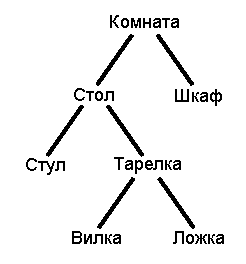
\includegraphics[width=0.5\textwidth]{pictures/child_parent_relationship.pdf}
        \caption{Иерархическое представление комнаты}
      \end{minipage}
  \end{figure}
  За основу решения взят основанный на правилах подход
  \begin{itemize}
    \item Ограничительная рамка и древовидное представление
    \item Входные табличные данные
    \item Рекурсивный алгоритм с возможностью удаления раннее расставленных объектов
  \end{itemize}
\end{frame}

\begin{frame}
  \frametitle{Особенности реализации}
  \begin{minipage}[m]{0.5\linewidth}
    \begin{figure}
      \centering
        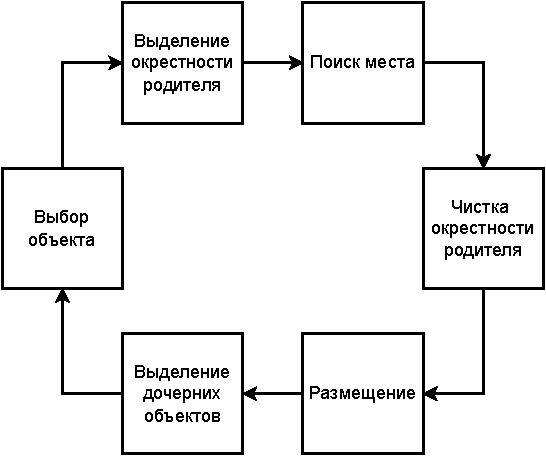
\includegraphics[width=\textwidth]{pictures/pcg.pdf}
        \caption{Последовательность шагов в алгоритме генерации интерьера}
    \end{figure}
    \end{minipage}\hfill
    \begin{minipage}[m]{0.5\linewidth}
      \begin{itemize}
        \item Использование F\# библиотеки в сторонних проектах на .NET
        \item Генератор псевдослучайных чисел
        \item Отдельные входные данные
        \item Алгоритм генерации без возможности удаления раннее расставленных объектов
      \end{itemize}
    \end{minipage}
\end{frame}

\begin{frame}
  \frametitle{Архитектура решения}
  \begin{figure}
    \centering
    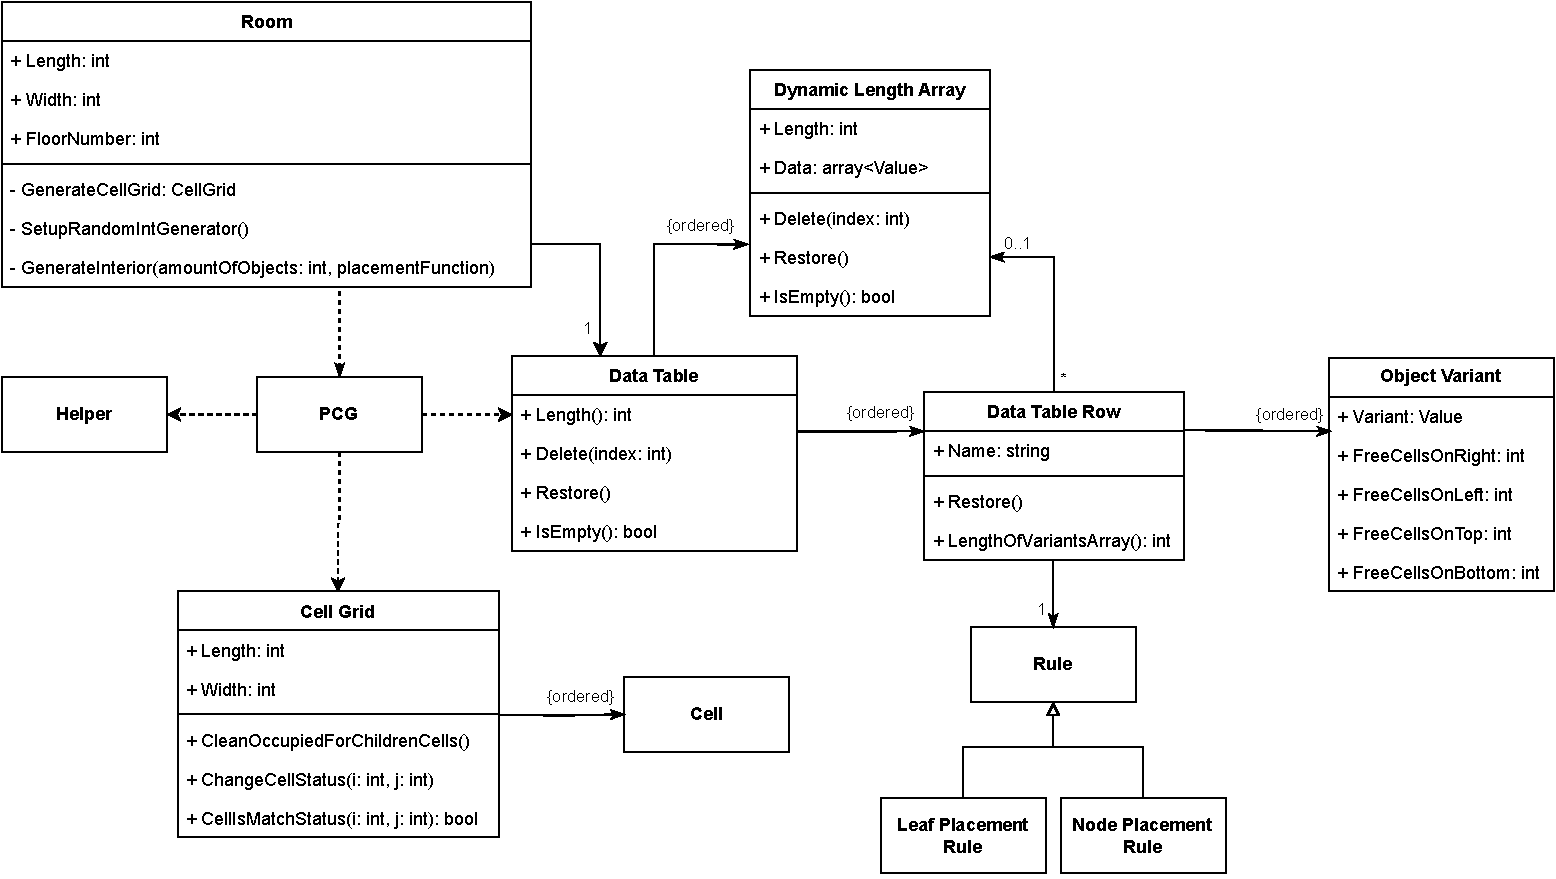
\includegraphics[width=0.8\textwidth]{pictures/uml.pdf}
    \caption{UML диаграмма классов реализованной библиотеки}
  \end{figure}
\end{frame}

\begin{frame}
  \frametitle{Интеграция в игру}
  \begin{minipage}[m]{0.6\linewidth}
    \begin{figure}
      \centering
        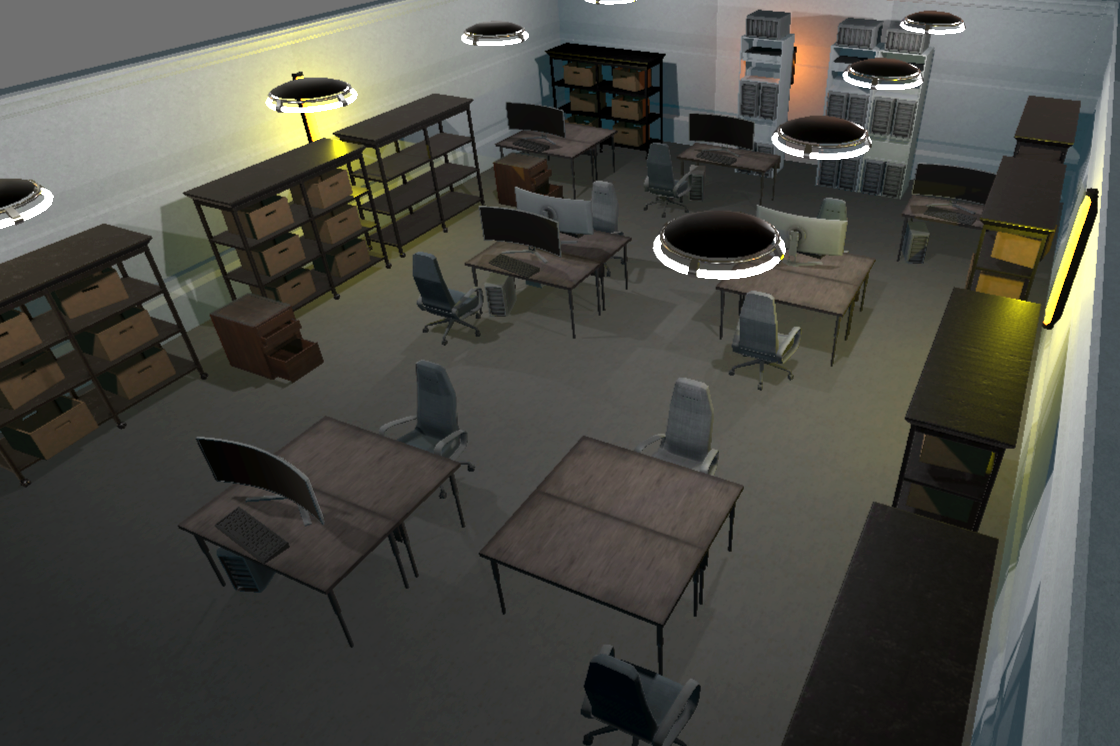
\includegraphics[width=\textwidth]{pictures/computing_center.png}
        \caption{Процедурно заполненный компьютерный центр}
    \end{figure}
    \end{minipage}\hfill
    \begin{minipage}[m]{0.4\linewidth}
      \begin{itemize}
        \item Логика в Unity Inspector
        \item Локальная координатная система
        \item Правила положения размещаемых объектов
      \end{itemize}
    \end{minipage}
\end{frame}

\begin{frame}
  \frametitle{Стороннее использование}
    \begin{figure}
      \centering
        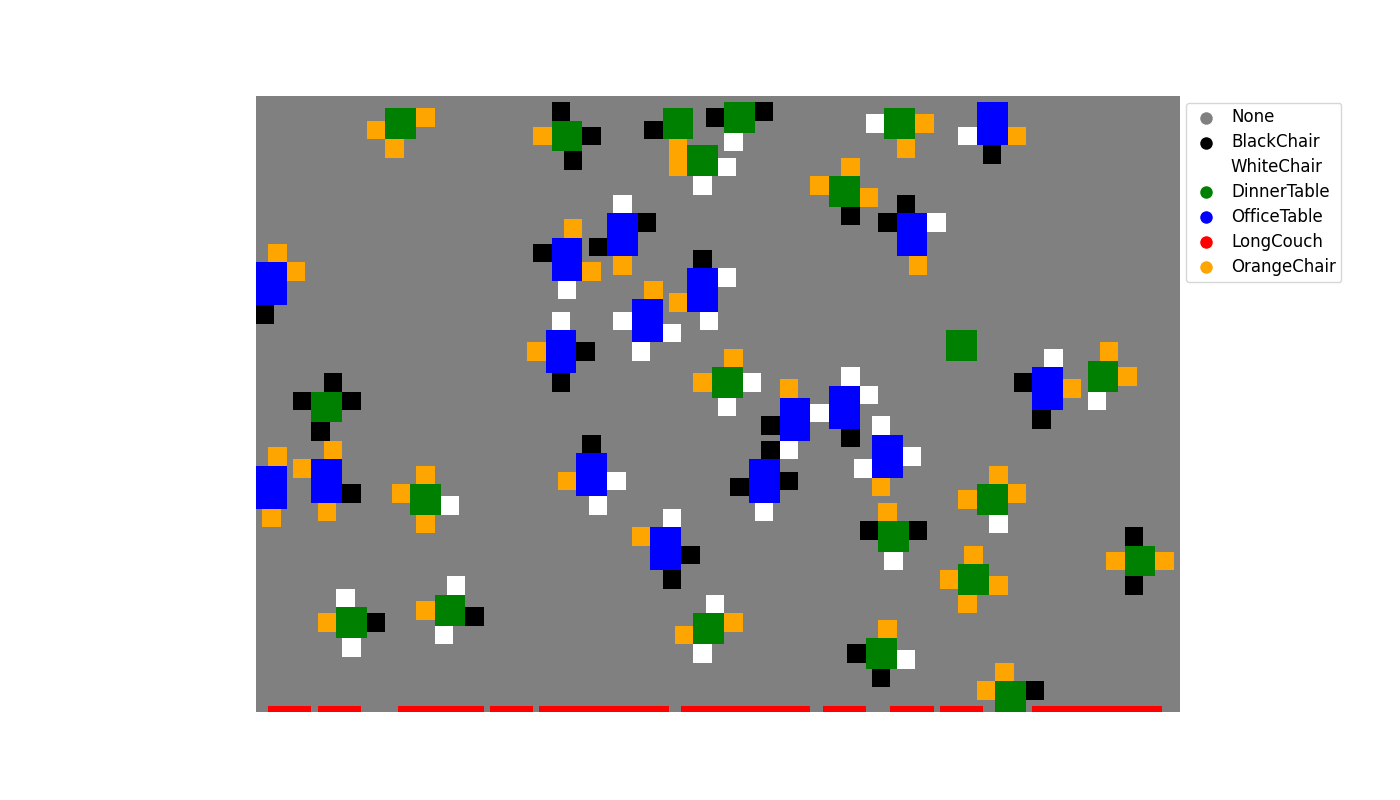
\includegraphics[width=\textwidth]{pictures/myplot.png}
        \caption{Процедурно заполненная двумерная комната}
  \end{figure}
\end{frame}

\begin{frame}[t]
  \frametitle{Апробация}
  %%\vspace*{\fill}
    \begin{itemize}
        \item Методика оценки качества продукта System Usability Scale
        \item В опросе приняли участие 13 человек  
        \item Средний балл по системе SUS составляет 68,1 при среднем показателе в 68 для систем, использующих данную систему оценивания
      \end{itemize} 
      \begin{figure}
      \centering
        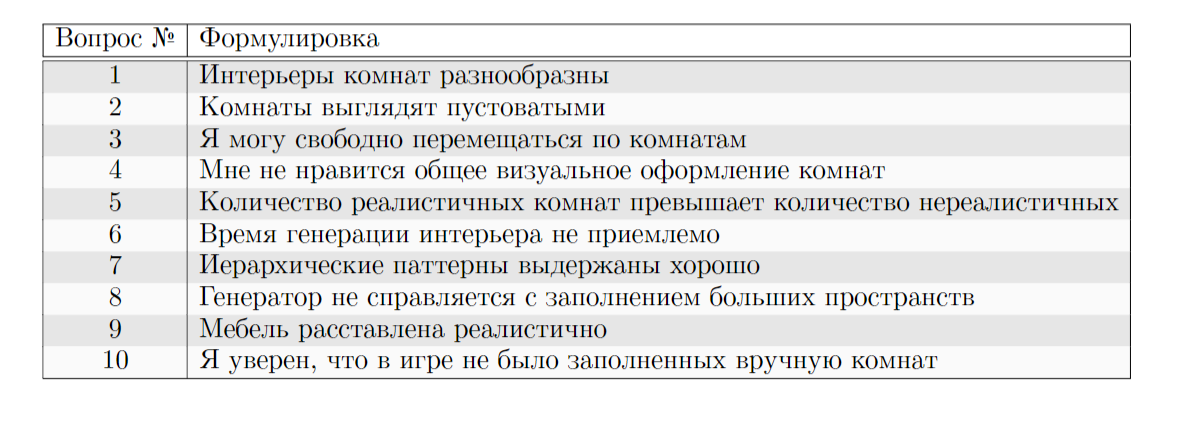
\includegraphics[width=\textwidth]{pictures/questions.png}
        \caption{Апробационные вопросы}
    \end{figure}
    %%\vspace*{\fill}
   
\end{frame}

\begin{frame}[t]
    \frametitle{Результаты апробации}
    \vspace*{\fill}
    \begin{figure}
      \centering
        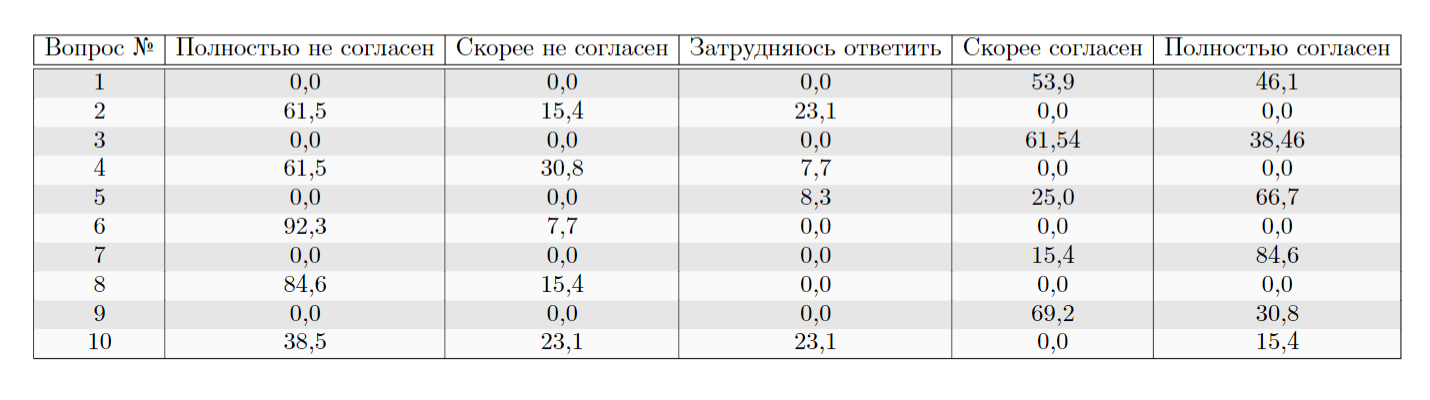
\includegraphics[width=\textwidth]{pictures/experiment.png}
        \caption{Процент участников, выбравших предложенные варианты}
    \end{figure}
    \vspace*{\fill}
\end{frame}

\begin{frame}
  \frametitle{Заключение}
    \begin{itemize}
        \item Рассмотрены существующие решения в области процедурной генерации интерьера комнат
        \item Реализована библиотека на .NET для генерации интерьера комнат, доступная для скачивания на платформе NuGet\footnote{NuGet: \url{https://www.nuget.org/packages/RoomInteriorGenerator}} и GitHub\footnote{GitHub: \url{https://github.com/PolinaSavelyeva/RoomInteriorGenerator}}
        \item Библиотека интегрирована в игру Ti\-me Re\-ac\-tor\footnote{Time Reactor: \url{https://github.com/RuslanBeresnev/Time-Reactor-Game}} на Uni\-ty En\-gi\-ne при помощи Uni\-ty Ins\-pec\-tor и C\# скриптов
        \item Проведена апробация среди заинтересованных игроков, которая подтвердила реалистичность генерируемых интерьеров и общую эффективность системы 
    \end{itemize}
\end{frame}

\end{document}